%% abtex2-modelo-relatorio-tecnico.tex, v-1.9.6 laurocesar
%% Copyright 2012-2016 by abnTeX2 group at http://www.abntex.net.br/ 
%%
%% This work may be distributed and/or modified under the
%% conditions of the LaTeX Project Public License, either version 1.3
%% of this license or (at your option) any later version.
%% The latest version of this license is in
%%   http://www.latex-project.org/lppl.txt
%% and version 1.3 or later is part of all distributions of LaTeX
%% version 2005/12/01 or later.
%%
%% This work has the LPPL maintenance status `maintained'.
%% 
%% The Current Maintainer of this work is the abnTeX2 team, led
%% by Lauro César Araujo. Further information are available on 
%% http://www.abntex.net.br/
%%
%% This work consists of the files abntex2-modelo-relatorio-tecnico.tex,
%% abntex2-modelo-include-comandos and abntex2-modelo-references.bib
%%

% ------------------------------------------------------------------------
% ------------------------------------------------------------------------
% abnTeX2: Modelo de Relatório Técnico/Acadêmico em conformidade com 
% ABNT NBR 10719:2015 Informação e documentação - Relatório técnico e/ou
% científico - Apresentação
% ------------------------------------------------------------------------ 
% ------------------------------------------------------------------------

\documentclass[
	% -- opções da classe memoir --
	12pt,				% tamanho da fonte
	openright,			% capítulos começam em pág ímpar (insere página vazia caso preciso)
	%twoside,			% para impressão em recto e verso. Oposto a oneside
	a4paper,			% tamanho do papel. 
	% -- opções da classe abntex2 --
	%chapter=TITLE,		% títulos de capítulos convertidos em letras maiúsculas
	%section=TITLE,		% títulos de seções convertidos em letras maiúsculas
	%subsection=TITLE,	% títulos de subseções convertidos em letras maiúsculas
	%subsubsection=TITLE,% títulos de subsubseções convertidos em letras maiúsculas
	% -- opções do pacote babel --
	english,			% idioma adicional para hifenização
	french,				% idioma adicional para hifenização
	spanish,			% idioma adicional para hifenização
	brazil,				% o último idioma é o principal do documento
	]{abntex2}



% PACOTES

% ---
% Pacotes fundamentais 
\usepackage{lmodern}			% Usa a fonte Latin Modern
\usepackage[T1]{fontenc}		% Selecao de codigos de fonte.
\usepackage[utf8]{inputenc}		% Codificacao do documento (conversão automática dos acentos)
\usepackage{indentfirst}		% Indenta o primeiro parágrafo de cada seção.
\usepackage{color}				% Controle das cores
\usepackage{graphicx}			% Inclusão de gráficos
\usepackage{microtype} 			% para melhorias de justificação
% ---

% Pacotes adicionais, usados no anexo do modelo de folha de identificação
\usepackage{multicol}
\usepackage{multirow}

\usepackage{float} % para utilizar o H de tabelas e figuras e mante-las no lugar
% ---

%----------------- PARA INSERIR ARQUIVOS DE CODIGOS -----------------%
\usepackage{xcolor}
% Definindo novas cores
\definecolor{verde}{rgb}{0,0.5,0}
% Configurando layout para mostrar codigos C++
\usepackage{listings}
\lstset{
  language=C, %indicar a linguagem utilizada
  basicstyle=\ttfamily\tiny, 
  keywordstyle=\color{blue}, 
  stringstyle=\color{verde}, 
  commentstyle=\color{gray}, 
  extendedchars=true, 
  showspaces=false, 
  showstringspaces=false, 
  numbers=left,
  numberstyle=\tiny,
  breaklines=true, 
  backgroundcolor=\color{green!10},
  breakautoindent=true, 
  captionpos=b,
  xleftmargin=0pt,
}
% -----------------% FIM INSERIR ARQUIVOs DE CODIGO -----------------%

% Pacotes de citações
\usepackage[brazilian,hyperpageref]{backref}	 % Paginas com as citações na bibl
\usepackage[num]{abntex2cite}	% Citações padrão ABNT
\citebrackets() %citação numérica entre colchetes
% --- 


% CONFIGURAÇÕES DE PACOTES

% Configurações do pacote backref
% Usado sem a opção hyperpageref de backref
\renewcommand{\backrefpagesname}{Citado na(s) página(s):~}
% Texto padrão antes do número das páginas
\renewcommand{\backref}{}
% Define os textos da citação
\renewcommand*{\backrefalt}[4]{
	\ifcase #1 %
		Nenhuma citação no texto.%
	\or
		Citado na página #2.%
	\else
		Citado #1 vezes nas páginas #2.%
	\fi}%
% ---


% Informações de dados para CAPA e FOLHA DE ROSTO
\titulo{Desenvolvimento de um ambiente tridimensional utilizando opengl}
\autor{João Pedro Miranda Miguel} %NAO PREENCHER
\local{São José dos Campos - Brasil}
\data{Dezembro de 2017}
\instituicao{
  Docente: Profª. Dra. Regina Célia Coelho
  \par
  Universidade Federal de São Paulo - UNIFESP
  \par
  Instituto de Ciência e Tecnologia - Campus São José dos Campos
}
\tipotrabalho{Relatório técnico}
\preambulo{Relatório apresentado à Universidade Federal de São Paulo como parte de um projeto desenvolvido na disciplina de computação gráfica.}
% ---

% Configurações de aparência do PDF final

% alterando o aspecto da cor azul
\definecolor{blue}{RGB}{41,5,195}

% informações do PDF
\makeatletter
\hypersetup{
     	%pagebackref=true,
		pdftitle={\@title}, 
		pdfauthor={\@author},
    	pdfsubject={\imprimirpreambulo},
	    pdfcreator={LaTeX with abnTeX2},
		pdfkeywords={abnt}{latex}{abntex}{abntex2}{relatório técnico}, 
		colorlinks=true,       		% false: boxed links; true: colored links
    	linkcolor=blue,          	% color of internal links
    	citecolor=blue,        		% color of links to bibliography
    	filecolor=magenta,      		% color of file links
		urlcolor=blue,
		bookmarksdepth=4
}
\makeatother
% --- 


% Espaçamentos entre linhas e parágrafos 

% O tamanho do parágrafo é dado por:
\setlength{\parindent}{1.3cm}

% Controle do espaçamento entre um parágrafo e outro:
\setlength{\parskip}{0.2cm}  % tente também \onelineskip

% compila o indice
\makeindex
% ---



% ------------------------------------------------
% Início do documento
\begin{document}

% Seleciona o idioma do documento (conforme pacotes do babel)
%\selectlanguage{english}
\selectlanguage{brazil}

% Retira espaço extra obsoleto entre as frases.
\frenchspacing 

% ----------------------------------------------------------
% ELEMENTOS PRÉ-TEXTUAIS
% ----------------------------------------------------------
% \pretextual

% ---
% Capa
\imprimircapa
% ---

% ---
% Folha de rosto
\imprimirfolhaderosto*
% ---

% ---
% RESUMO
% resumo na língua vernácula (obrigatório)
\setlength{\absparsep}{18pt} % ajusta o espaçamento dos parágrafos do resumo
\begin{resumo}
Esse relatório pretende discorrer sobre o projeto de um ambiente tridimensional contendo um personagem animado que apresenta interação com o usuário. Esse projeto foi realizado como parte da disciplina de computação gráfica da universidade federal de São Paulo campus São José dos Campos. O objetivo do projeto é então projetar um ambiente tridimensional que contenha ao menos um personagem responsável por realizar alguma tarefa. Nesse projeto optou-se por fazer algo inspirado em alguns jogos de fazenda onde o fazendeiro, que é o personagem, se movimenta e planta algo conforme o local do ambiente em  que houve o \emph{click} do \emph{mause}. Nesse projeto deverá haver também uma opção para que o personagem ande pelo cenário e cumpra uma animação pré definida de forma autônoma, isto é, sem esperar uma entrada do usuário. Além disso deverá haver também opções para se movimentar cada parte do corpo do personagem separadamente. Todo esse projeto é desenvolvido utilizando visão perspectiva e implementado utilizando-se o pacote gráfico opengl. 


 \noindent
 \textbf{Palavras-chaves}: opengl, ambiente tridimensional, computação gráfica.
\end{resumo}

%------LISTAS SÃO OPCIONAIS---------
% inserir lista de ilustrações
%\pdfbookmark[0]{\listfigurename}{lof}
%\listoffigures*
%\clearpage

% inserir lista de tabelas
%\pdfbookmark[0]{\listtablename}{lot}
%\listoftables*
%\clearpage
% ---

%SUMÁRIO É OBRIGATÓRIO
% inserir o sumario
\pdfbookmark[0]{\contentsname}{toc}
\tableofcontents*
% ---


% ----------------------------------------------------------
% ELEMENTOS TEXTUAIS
\textual

% ----------------------------------------------------------
\chapter{Introdução}

Um dos fatores decisivos para a popularização dos computadores foi a invenção da interface gráfica. Graças a isso tornou-se possível, para alguém sem conhecimentos profundos sobre o funcionamento dos computadores ou de alguma linguagem de programação, utilizá-lo sem muito sofrimento. Com a popularização dos computadores e os avanços no poder de processamento tornou-se então possível a criação de ambientes gráficos virtuais tridimensionais para as mais variadas funções. 

 %O que seria das tardes de domingo sem os jogos eletrônicos ou dos filmes de ação e ficção sem os efeitos especiais ? Nossas infâncias não teriam sido as mesmas sem os filmes de desen 
  
Pode-se citar como aplicações, das técnicas envolvidas na criação de ambientes gráficos virtuais, a criação de  jogos eletrônicos, a aplicação de efeitos especiais em filmes entre várias outras como por exemplo a plicação em simulações médicas a fim de melhor preparar os médicos para fazer uma cirurgia. 

Visando então desenvolver habilidades práticas no desenvolvimento de aplicações gráficas, foi feito um projeto onde o objetivo era ter um humanóide em um cenário e que esse humanóide tivesse alguma função no ambiente em que ele estivesse inserido. Nesse projeto optou-se por fazer algo inspirado nos jogos de fazenda onde uma das funções do personagem é plantar. Então nesse projeto foi desenvolvido um ambiente tridimensional com um personagem em opengl onde, o personagem tem por objetivo plantar em todos os lugares do cenário em que houve um \emph{click} do \emph{mause}. Também foram incluidas opções para se movimentar cada parte do personagem e para executar uma animação automática que não depende de nenhuma entrada do usuário.

%Palavras estrangeiras como \emph{hardware} devem ser destacadas.
%-------------------------------------------------------------------------------------------------------------------------INTRODUCAO



%------------------- MODELO DE FIGURA -----------------------------
%Modelo da \autoref{fig:esquematico}:
%\begin{figure}[H]
%\centering 
%\caption{Esquematico} \label{fig:esquematico}
%\includegraphics[scale=0.3]{esquematico.png}
%\legend{Fonte: Computer Organization and Design  }
%\end{figure}


%------------------- MODELO DE TABELA -----------------------------
%Modelo da \autoref{tab:Instr3OP}:
%\begin{table}[htb]
%\centering
%\ABNTEXfontereduzida
%\caption{Exemplo de um formato de Instruções} \label{tab:Instr3OP}
%\begin{tabular}{r|p{2cm}|p{1.7cm}|p{1.7cm}|p{1.7cm}|p{3cm}} 
%\textbf{Tamanho (bits)} & 6 & 5 & 5 & 5 & 11 \\ \hline
%\textbf{Campo} & OPcode & Reg1 & Reg2 & Reg3 & Blank \\ \hline
%\textbf{Bits} & 31 - 26 & 25 - 21 & 20 - 16 & 15 - 11 & 10 - 0\\
%\end{tabular}
%\legend{Fonte: O Autor}
%\end{table}

%Como utilizar \textbf{Anexos}
%Material que não seja de autoria própria que traga maiores detalhes de algo utilizado no decorrer do relatório

%Como utilizar \textbf{Apêndices}
%Material de autoria própria que traga maiores detalhes e que não seja essencial no decorrer do relatório.

%Modos de comandos $\backslash$ref\\
%$\backslash$ref: \ref{fig:esquematico}\\
%$\backslash$nameref: \nameref{fig:esquematico}\\
%$\backslash$autoref: \autoref{fig:esquematico}\\

%Existe uma forma de inserir arquivos de códigos diretamente no latex, verificar a formatação nas linhas 70 a 93 do código latex e a inserção feita do código \nameref{code:BinToBCD2.v} no \autoref{code:BinToBCD2.v} 

\chapter[Objetivos]{Objetivos}

	 Foi proposto no projeto desenvolver um ambiente gráfico tridimensional com um personagem que realizará uma tarefa. Inspirado em jogos de fazenda e no popular título "minecraft" tem-se então como meta desenvolver um ambiente rural e um humanóide que irá plantar algo a depender do lugar em que houve algum \emph{click} do  \emph{mause}.

	Também será implementada as opções de se ativar uma animação automática e de mover cada parte do humanóide. Na animação automática o humanóide irá dançar seguindo uma sequência de passos e andará pelo cenário, já na opção para se movimentar cada parte do humanóide será permitido escolher qual parte do corpo mover e esse movimento será realizado observando as limitações fisicas de um ser humano real.  


\chapter{Metodologia}

	A seguir é apresentado como foi desenvolvida cada parte do projeto e na secção \ref{subsec:dependencias} é falado sobre o que é necessário para se compilar e rodar o programa.

 \section{Cenário}
	
	Tendo em mente que o personagem seria um fazendeiro e que teria como tarefa plantar, foi feito um ambiente, em céu aberto contendo árvores e uma casa simples, que remete à uma área rural. Para fazer a casa, as árvores, o chão e o céu utilizou-se de formas geométricas primitivas, no caso esferas e cubos.

	No caso do céu optou-se por fazer uma esfera de cor azul englobando todo o cenário. O chão foi feito com um cubo  bem grande transladado para baixo. As árvores foram feitas combinando-se esferas e cubos e a casa foi feita combinando-se cubos e triângulos.

No caso do chão e da casa foi necessário fazer funções para desenhar as formas geométricas de modo a poder se inserir textura. Foram feitas funções para se desenhar um cubo utilizando-se do conceito de \emph{sweep} visto em aula para se determinar os vértices do cubo e utilizando o comando \emph {glTesxCoord2f } para se definir cada cordenada de textura do cubo. Foram feitas três funções diferentes para se desenhar cubos.

Duas das funções desenham um cubo com uma única textura repetindo ela em todas as faces do mesmo, a diferença é em como as cordenadas de textura são definidas, enquanto que em uma das funções o cubo tem cordenadas de textura de 0 a 1, na outra o cubo tem cordenadas de textura de 0 a 50. A segunda função foi criada para se mapear a textura no chão de forma a fazer com que a textura se repetisse várias vezes tendo em vista o tamanho pequeno da textura em relação ao tamanho do chão.

A outra função que desenha um cubo com textura única foi utilizada para se desenhar a casa que não precisava de repetição de textura devido ao tamanho da textura em relação à casa, essa função também foi utilizada para se desenhar o solo onde o personagem planta como é dito com maiores detalhes na secção \ref{subsec:planta}  e para se desenhar algumas partes do personagem como é dito na secção  \ref{subsec:personagem}. 

A outra função para desenhar cubos desenha um cubo com seis texturas diferentes, uma em cada face, e foi utilizada para  se desenhar algumas partes do humanóide, ela é explicada com maiores detalhes na secção \ref{subsec:personagem}.

Para se montar as árvores e a casa utilizou-se de transformações geométricas para se posicionar os cubos e esferas de modo a formar as árvores e a casa.  Para se montar o telhado da casa utilizou-se de cálculos trigonométricos a fim de definir os ângulos de rotação necessários para se posicionar as laterais do telhado, os cálculos foram  feitos defindo-se um triângulo isósceles como sendo o formato do telhado. Já os triângulos frontais do telhado foram posicionados utilizando-se de translações.

Foram feitos dois tipos de árvores, um foi obtido através da combinação de cubos e esferas e o outro através da combinação de cones e cubos. Foi utilizado de tranformações geométricas tais como escala e translação para se pocionar cada elemento das árvores a fim de se obter o resultado final.

Por fim, para se montar o cenário, foi feita uma função que define posições aleatórias onde serão desenhas um determinado número de árvores de cada tipo. Essa função também é reponsável por definir possições onde serão desenhadas algumas plantas e solos como é dito na secção \ref{subsec:planta}. Essas posições são salvas em filas que são utilizadas todas as vezes que a tela tem que ser redesenhada para se definir onde desenhar as árvores e os solos e plantas.

 

   
  

 


\section{Personagem}
\label{subsec:personagem}

 Inspirado no jogo popular "minecraft" o personagem foi desenhado através de cubos que foram transladados e sofreram transformações de escala afim de formar o personagem. Foram adicionadas esferas em cada articulação para que não ficassem buracos quando o personagem executasse alguma animação. Todo o personagem foi construido utilizando-se o conceito de hierarquia visto em sala com o intuito de se fazer as movimentações do personagem de modo coerente com a relaidade. 

Para se desenhar os cubos que formam a cabeça e o tronco do personagem foi feita um função que desenha um cubo com uma textura diferente em cada face a fim de se representar o rosto e a parte central das roupas do personagem. Os braços, pernas, pés, mãos e pescoço foram desenhados utilizando-se de uma função que desenha cubos com uma única textura repetindo ela em todas as faces do cubo. As texturas são passadas como argumento dessas funções através de vetores que contém os identificadores de cada textura. As funções criadas para desenhar os cubos com textura também definem as normais para cada face do cubo necessárias para os cálculos de iluminação relaizadas pelo opengl.

Utilizando-se do conceito de objetos filhos foi também criado uma enxada através de cubos e transformações geométricas que foi ligada como objeto filho das mãos do personagem. A enxada se encontra por hierarquia atada as mão do personagem e só é desenhada  se uma determinada condição é satisfeita o que faz com que seja possível controlar quando e em que mão a enxada é desenhada ou não. 
    


\section{Solos e plantas}
\label{subsec:planta}
	
	Quando há um \emph{cilck} na tela, aparece um solo no chão no lugar onde houve o \emph{click}. Depois de aparecer o solo o personagem se movimenta até o local e planta uma planta. Apartir dai o solo é então desenhado com uma planta em cima. Para se obter esse resultado o solo e a planta foram criados utilizando-se do conceito de objeto filho onde a planta é atada como objeto filho do solo e só é desenhada se uma determinada condição é satisfeita.
 	O solo foi desenhado como um cubo com transformações de escala e de translação. Para se desenhar o cubo do solo utilizou-se da função criada para se desenhar cubos com uma única textura. As plantas foram desenhadas através de cubos e esferas, com transformações de escala e de translação. As esferas no topo das plantas foram desenhadas com cores aleatórias de modo a simular flores diferentes.
  


\section{Texturas}

	As texturas foram carregadas utilizando-se uma biblioteca chamada SOIL que facilita o carregamento das mesmas. Os vetores com os identificares de cada textura carregada foram declarados como variáveis globais. Dentro das funções feitas para se criar cubos com textura são feitas chamadas para a função \emph{glBindTexture} para que se defina que textura será aplicada sobre cada face do cubo. 

	No carregamento das texturas foi definido para que o opengl aplique os filtros de aumento e diminuição linear de textura. Na função feita para se desenhar um cubo com única textura utilizada para se fazer o chão  foi definido também que o opengl faça a repetição das texturas nos eixos x e z. 
	
\section{Animações}
	
Foram feitas três animações distintas, a do personagem andando, plantando e dançando. Cada uma dessas animações é guardada em uma fila através das posições do personagem e dos ângulos que cada membro do corpo do personagem deve girar a cada quadro. Todas as animações são calculadas em relação a posição atual do personagem sempre que ele necessita de executar alguma delas.


Para tanto foram feitas três funções, uma para cada animação, reponsáveis por calcular a posição do personagem e os ângulos que cada parte do corpo do personagem deverá girar a cada quadro desenhado. Esses ângulos e  posições são então armazenados em filas que são percorridas para executar a animação. As posições são utilizadas para se fazer translações e os âgulos as rotações necessárias a cada quadro a fim de se executar a animação.

A função que faz a animação do personagem andando também é responsável por calcular uma trajetória para que o personagem se desloque enquanto executa a animação de andar. Essa trajetória é calculada através do conceito de  variação,  visto em física, do ponto final para onde o personagem deverá se deslocar em relação ao ponto inicial de onde o personagem irá partir. A partir dessa variação é calculado então o quanto o personagem deverá andar no eixo x e no eixo z afim de chegar no destino.

	Apartir disso é calculado a posição do personagem a cada quadro bem como a quantidade de passos que ele deverá dar nas direções dos eixos x e z.
Para se calcular os ângulos das pernas do persongem e o tanto que ele deverá transladar, para baixo quando ele dobra o joelho ou para frente quando ele dobra a perna para trás,  foram utilizadas relações trigonométricas. 

	Para a execução das animações foram feitas funções que percorrem as filas onde foram guardadas as animações e desenham o personagem na posição e com os ângulos descritos. O tempo das animações é dado pelo tempo que é definido para a função esperar entre o desenho de cada quadro.  
	 
\section{Câmera}

	As opções de movimentação da câmera foram feitas com base em uma circunferência de raio 0.2, onde o foco da câmera se encontra em algum ponto sobre a circunferência e a origem da circunferência é a posição da câmera. Para se descrever os pontos da circunferência utilizou-se das equações paramétricas da circunferência.

Quando as teclas 'a' e 'd' são pressionadas é somado, ao local da câmera e ao ponto focal, o ponto que está a 90 graus, positivos se a tecla for 'a' e negativos se a tecla for 'd', do foco da câmera na circunferência. Isso faz com que a câmera sempre se desloque a uma distancia do tamanho do raio da circunferencia sempre que essas teclas são precionadas. Isso faz com que a câmera se desloque para os lados esquedo e direito.

Para a câmera se deslocar para frente e para trás, quando pressionadas as teclas 'w' e 's', foi feita a soma da origem da circunferência e do ponto focal com o ponto onde se encontra o foco no caso da tecla 'w' e com o ponto que se encrontra a menos 180 graus do ponto de foco no caso de ser a tecla 's'. Isso faz com que a câmera se desloque para frente e para trás sempre percorrendo distancias iguais ao tamanho do raio sempre que alguma dessas teclas são pressionadas.         

Para se fazer o giro da câmera, quando pressionadas as teclas 'q' e 'e', o ponto focal é deslocado sobre a circunfêrencia em mais 1,8 graus quando a tecla pressionada é 'q' e em menos 1,8 graus quando a tecla pressionada é 'e'. Isso faz com que a câmera gire no sentido anti-horário e no sentido horário.

\section{Iluminação}

	Tendo em mente que se queria fazer o ambiente de modo que desse a entender que estivesse amanhecendo, foram utilizadas duas fontes de luz posicionadas próximas uma da outra de modo que se encontrassem perto de uma das extremidades do cenário e acima do chão. As caracteristicas de cada fonte, isto é a instensidade de luz ambiente, especular e difusa, foram definidas de modo semelhante para as duas fontes. Optou-se pelo uso de duas fontes para se obter um efeito melhor de iluminação que não foi alcançado com uma única fonte. 

Para que as fontes de luz ficassem imóveis conforme movimenta-se a câmera, toda as vezes que a câmera é movida, são feitas chamadas para a função \emph{glLightfv} que define sempre a mesma posição para as fontes de luz. Isso é necessário porque no opengl as informações da posição das luzes são guardadas juntamente com as informações da câmera, o que faz com que quando a câmera sofra alguma mudança as luzes também o sofram.    	

\section{Reconhecimento dos \emph{clicks} do mause}

	Para que fosse reconhecido o local do ambiente correspondente ao local em que houve o \emph{click} do \emph{mause} na tela, foram aplicadas as transformações inversas das que o opengl aplica para calcular a projeção do modelo na tela. Para tanto os pontos da tela onde houve \emph{clicks} do \emph{mause} tiveram seus valores de y invertidos para serem compativeis com o sistema de cordenadas do opengl, depois os pontos foram normalizados e multiplicados pelas matrizes inversas das matrizes de projeção e de modelo do opengl. Como cordenada z da tela foi utilizado o valor do \emph{depth buffer} no ponto x, y em que houve o \emph{click}  do \emph{mause}.  	


\section{Menus}

	Os menus que aparecem com o click do botão direito do mause foram feitos com o auxilio das funções \emph{glutCreateMenu}, \emph{glutAddSubMenu} e \emph{glutAddMenuEntry}. Na implementação optou-se por fazer o controle do programa através desses menus de modo que cada opção altera os valores de algumas variáveis globais reponsáveis por dizer ao programa como ele deve prosseguir. 

   
\section{Dependências}
\label{subsec:dependencias}
	
Para se compilar o programa desenvolvido é necessário ter instalado, além das bibliotecas padrões da linguagem c e da glu e glut do opengl, a biblioteca SOIL utilizada para o carregamento de texturas. Para se executar o programa é necessário haver uma pasta, no mesmo diretório do executável, com o nome texturas onde deverão ser armazenadas as texturas que serão utilizadas pelo programa.

Para a instalação da biblioteca SOIL é necessário adicionar o compilado dessa biblioteca dentro da pasta que contém as bibliotecas do compilador. Também é necessário adicionar o arquivo '.h' da SOIL na pasta que contém os arquivos '.h' do compilador. Para a compilação desse projeto foi utilizado o compilador GCC no sistema operacional windows. Para se obter a biblioteca SOIL recomenda-se o site \url{http://www.lonesock.net/soil.html}.

       
\chapter{Resultados e Discussões}
	A \autoref{arvorecomcone} e a \autoref{arvorecomesferas} mostram os dois tipo de árvores construidas para fazer parte do cenário, a árvore da \autoref{arvorecomcone} foi construida combinando-se cubos e cones com transformações de escala e de translação. Já a árvore da \autoref{arvorecomesferas} foi construida combinando-se esferas e cubos. 

\begin{figure}[H]
\centering 
\caption{Árvore feita apartir da combinação de cones e cubos} \label{arvorecomcone}
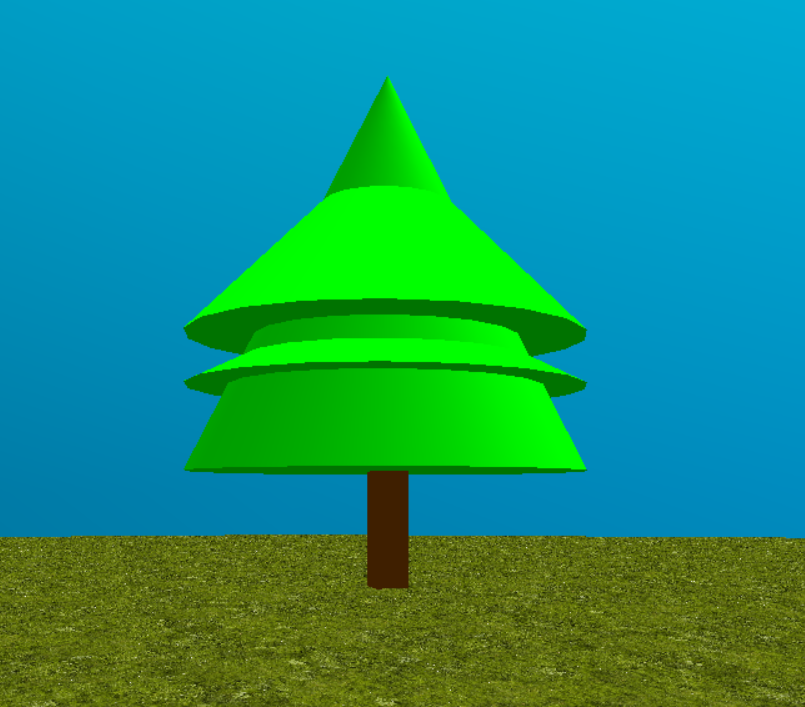
\includegraphics[scale=0.5]{imagens/arvorecomcones.png}
\legend{Fonte: o autor}
\end{figure}

\begin{figure}[H]
\centering 
\caption{Árvore feita apartir da combinação de esferas e cubos} \label{arvorecomesferas}
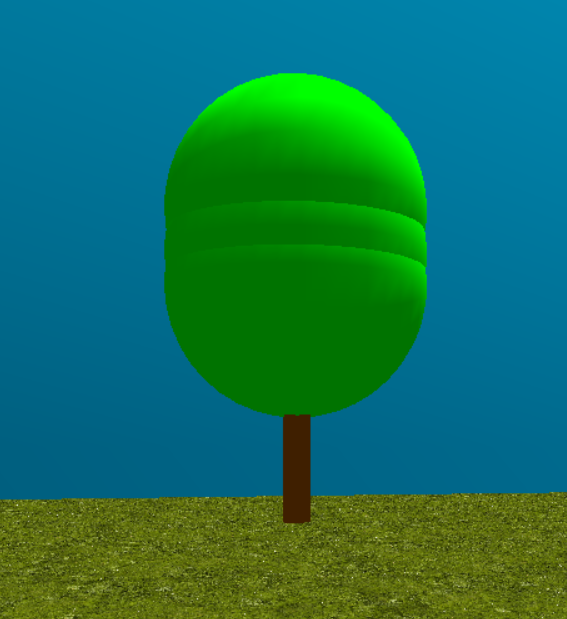
\includegraphics[scale=0.5]{imagens/arvorecomesferas.png}
\legend{Fonte: o autor}
\end{figure}

	A \autoref{casa} e a \autoref{casa2} mostram a casa que foi construida através da combinação de cubos, triângulos e algumas texturas.

\begin{figure}[H]
\centering 
\caption{Casa feita apartir da combinação de cubos e triângulos } \label{casa}
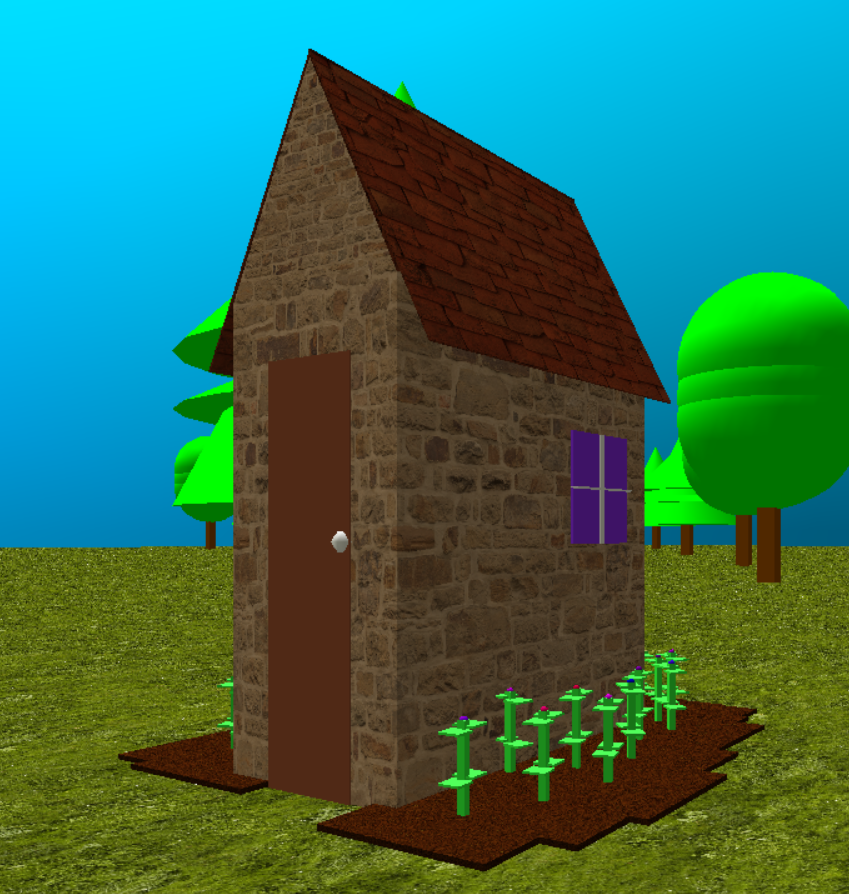
\includegraphics[scale=0.6]{imagens/casa.png}
\legend{Fonte: o autor}
\end{figure}

\begin{figure}[H]
\centering 
\caption{Casa feita apartir da combinação de cubos e triângulos } \label{casa2}
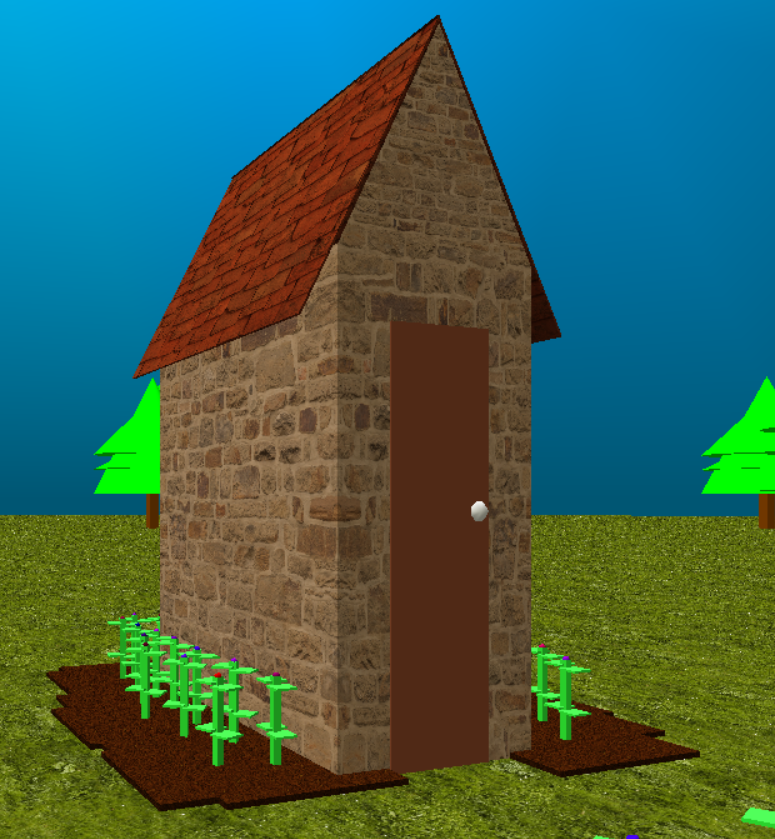
\includegraphics[scale=0.6]{imagens/casa2.png}
\legend{Fonte: o autor}
\end{figure}

	A \autoref{solo} mostra o que aparece ao \emph{click} do \emph{mause}. Definiu-se para esse objeto o nome de solo e ele foi criado através de um cubo com textura. A \autoref{solocomplanta} mostra o solo logo após o personagem cultivá-lo. Nesse momento aparece no centro do solo uma planta que  foi construida através de cubos e esferas. As esferas no topo das plantas tem cores definidas aleatóriamente.
  
\begin{figure}[H]
\centering 
\caption{Solo que aparece ao \emph{click} do \emph{mause} } \label{solo}
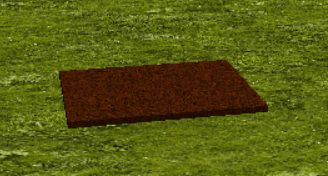
\includegraphics[scale=1]{imagens/solo.png}
\legend{Fonte: o autor}
\end{figure}

\begin{figure}[H]
\centering 
\caption{Solo com a planta } \label{solocomplanta}
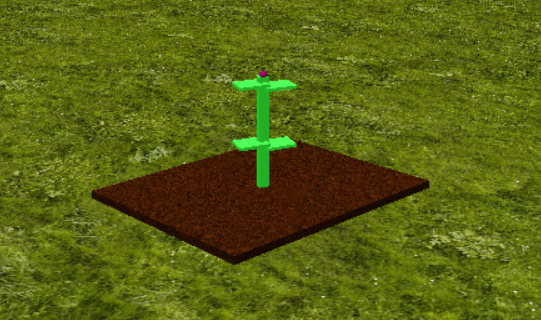
\includegraphics[scale=1]{imagens/solocomplanta.png}
\legend{Fonte: o autor}
\vspace{-1.5em}

\end{figure}




A \autoref{personagemfig} mostra o persongem, no caso um fazendeiro, que foi construido apartir de cubos com textura que foram escalonados e transladados. Em cada articulação do personagem foram inseridas esferas para que não aparecessem buracos quando o personagem movesse alguma parte do corpo. Isso pode ser visto na \autoref{movimentopersonagem}, nessa figura é também mostrado o que acontece quando é selecionada alguma opção no menu para se movimentar o personagem, quando isso acontece o personagem é desenhado em um cenário diferente e as setas do teclado podem então ser utilizadas para se movimentar a parte do personagem que foi selecionada.

\begin{figure}[H]
\centering 
\caption{Personagem feito com cubos ao estilo minecraft} \label{personagemfig}
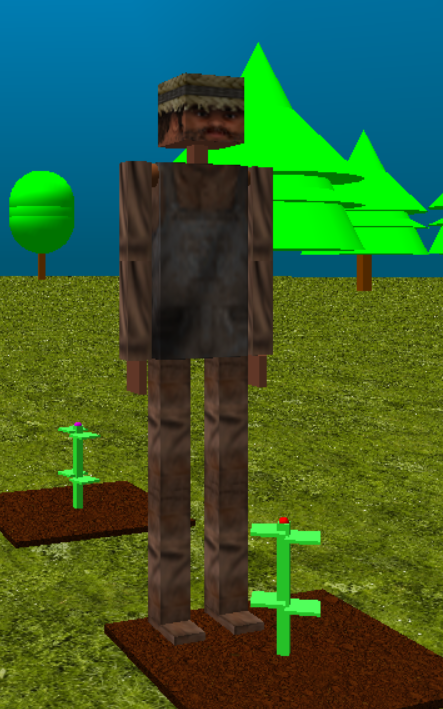
\includegraphics[scale=0.6]{imagens/personagem.png}
\legend{Fonte: o autor}
\end{figure}


\begin{figure}[H]
\centering 
\caption{Movimentos do personagem sendo feito pelas setas do teclado} \label{movimentopersonagem}
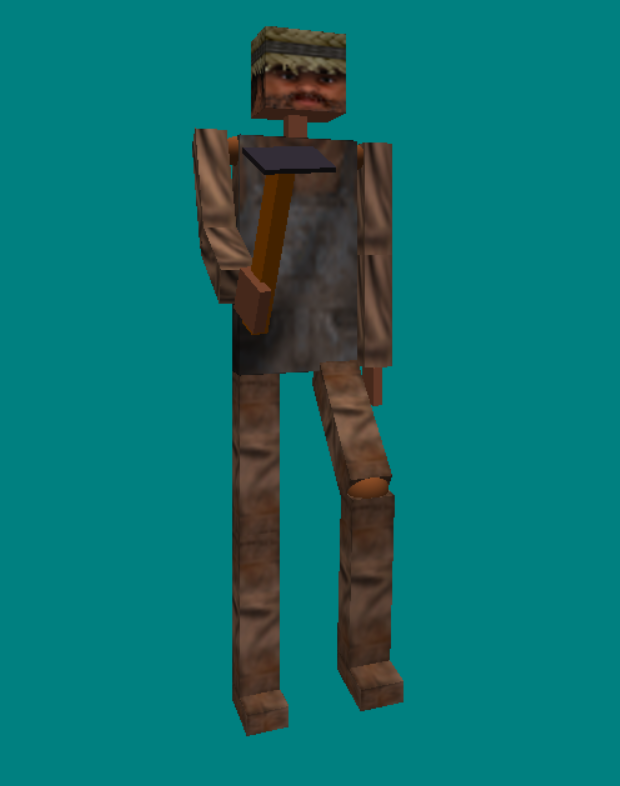
\includegraphics[scale=0.6]{imagens/movimentopersonagem.png}
\legend{Fonte: o autor}
\end{figure}



	A \autoref{menu} mostra o menu que aparece na tela ao \emph{click} do botão direito do \emph{mause}, nesse menu há as opções para se mover o personagem, que abre um submenu para se selecionar que parte do personagem movimentar, para executar a animação automática onde o personagem dança e anda pelo cenário, para o modo jogo onde o programa reconhece os \emph{clicks} do botão esquerdo do \emph{mause} como sendo os lugares em que o personagem tem  que ir plantar e, por último a opção para se resetar o jogo onde as plantas que foram plantadas são excluidas e o programa começa a executar denovo como se tivesse sido acabado de ser inicializado, setando a posição do personagem e da câmera  para a posição inicial.  

	A \autoref{menu2} e \autoref{menu3} mostram os submenus referentes a opção de mover o personagem presente no menu principal. 
\begin{figure}[H]
\centering 
\caption{Menu principal  } \label{menu}
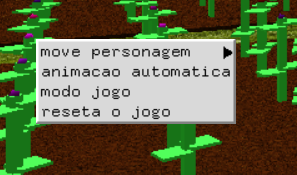
\includegraphics[scale=0.8]{imagens/menudeopcoes.png}
\legend{Fonte: o autor}
\end{figure}

\begin{figure}[H]
\centering 
\caption{Menu principal com submenu de opções para se movimentar o personagem } \label{menu2}
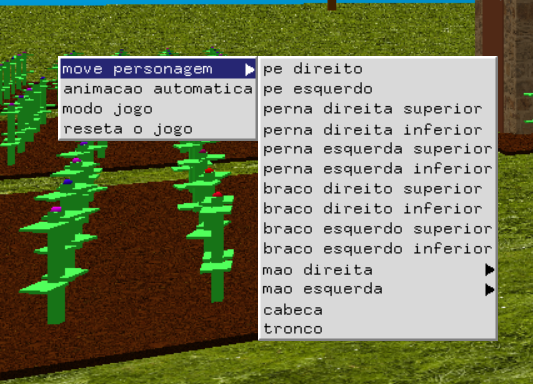
\includegraphics[scale=0.8]{imagens/menudeopcoes2.png}
\legend{Fonte: o autor}
\end{figure}

\begin{figure}[H]
\centering 
\caption{Menu principal com submenu de opções para se movimentar o personagem mostrando as opções de se movimentar as mão do personagem com ou sem a exada } \label{menu3}
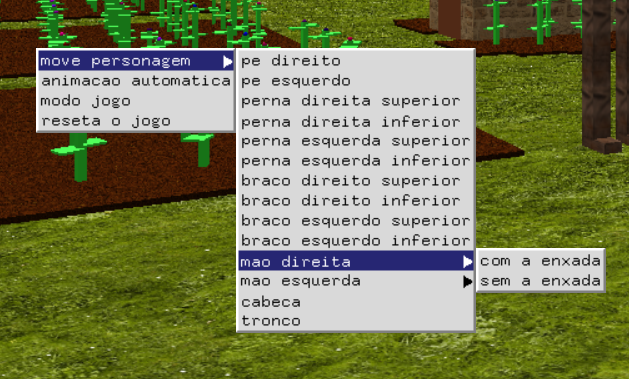
\includegraphics[scale=0.8]{imagens/menudeopcoes3.png}
\legend{Fonte: o autor}
\end{figure}

	A \autoref{enxada} mostra a enxada que aparece na mão do personagem quando este esta plantando ou quando é selecionado no menu de opções para se movimentar a mão do personagem com a enxada.

\begin{figure}[H]
\centering 
\caption{Enxada que aparece na mão do personagem } \label{enxada}
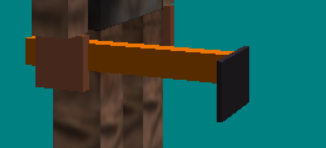
\includegraphics[scale=0.8]{imagens/enxada.png}
\legend{Fonte: o autor}
\end{figure}

 A \autoref{cenario} e \autoref{cenario2} mostram como ficou o o cenário  depois de montado com os elementos já descritos aqui. Nessas imagens também da para ver melhor como ficou o chão com a textura e o céu com a iluminação de duas fontes de luz próximas uma da outra. 

\begin{figure}[H]
\centering 
\caption{Cenário construido } \label{cenario}
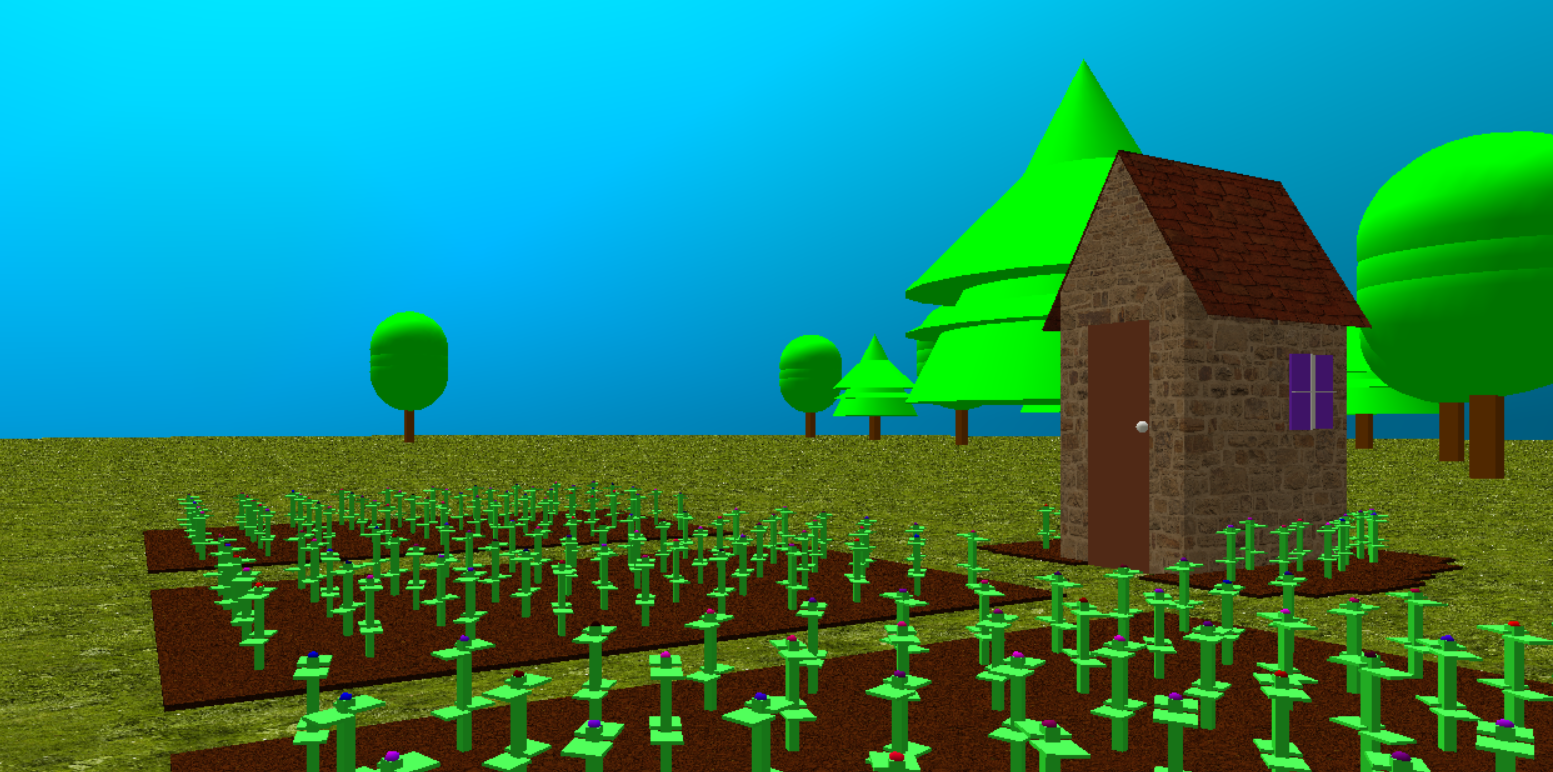
\includegraphics[scale=0.4]{imagens/cenario.png}
\legend{Fonte: o autor}
\end{figure}

\begin{figure}[H]
\centering 
\caption{Cenário construido } \label{cenario2}
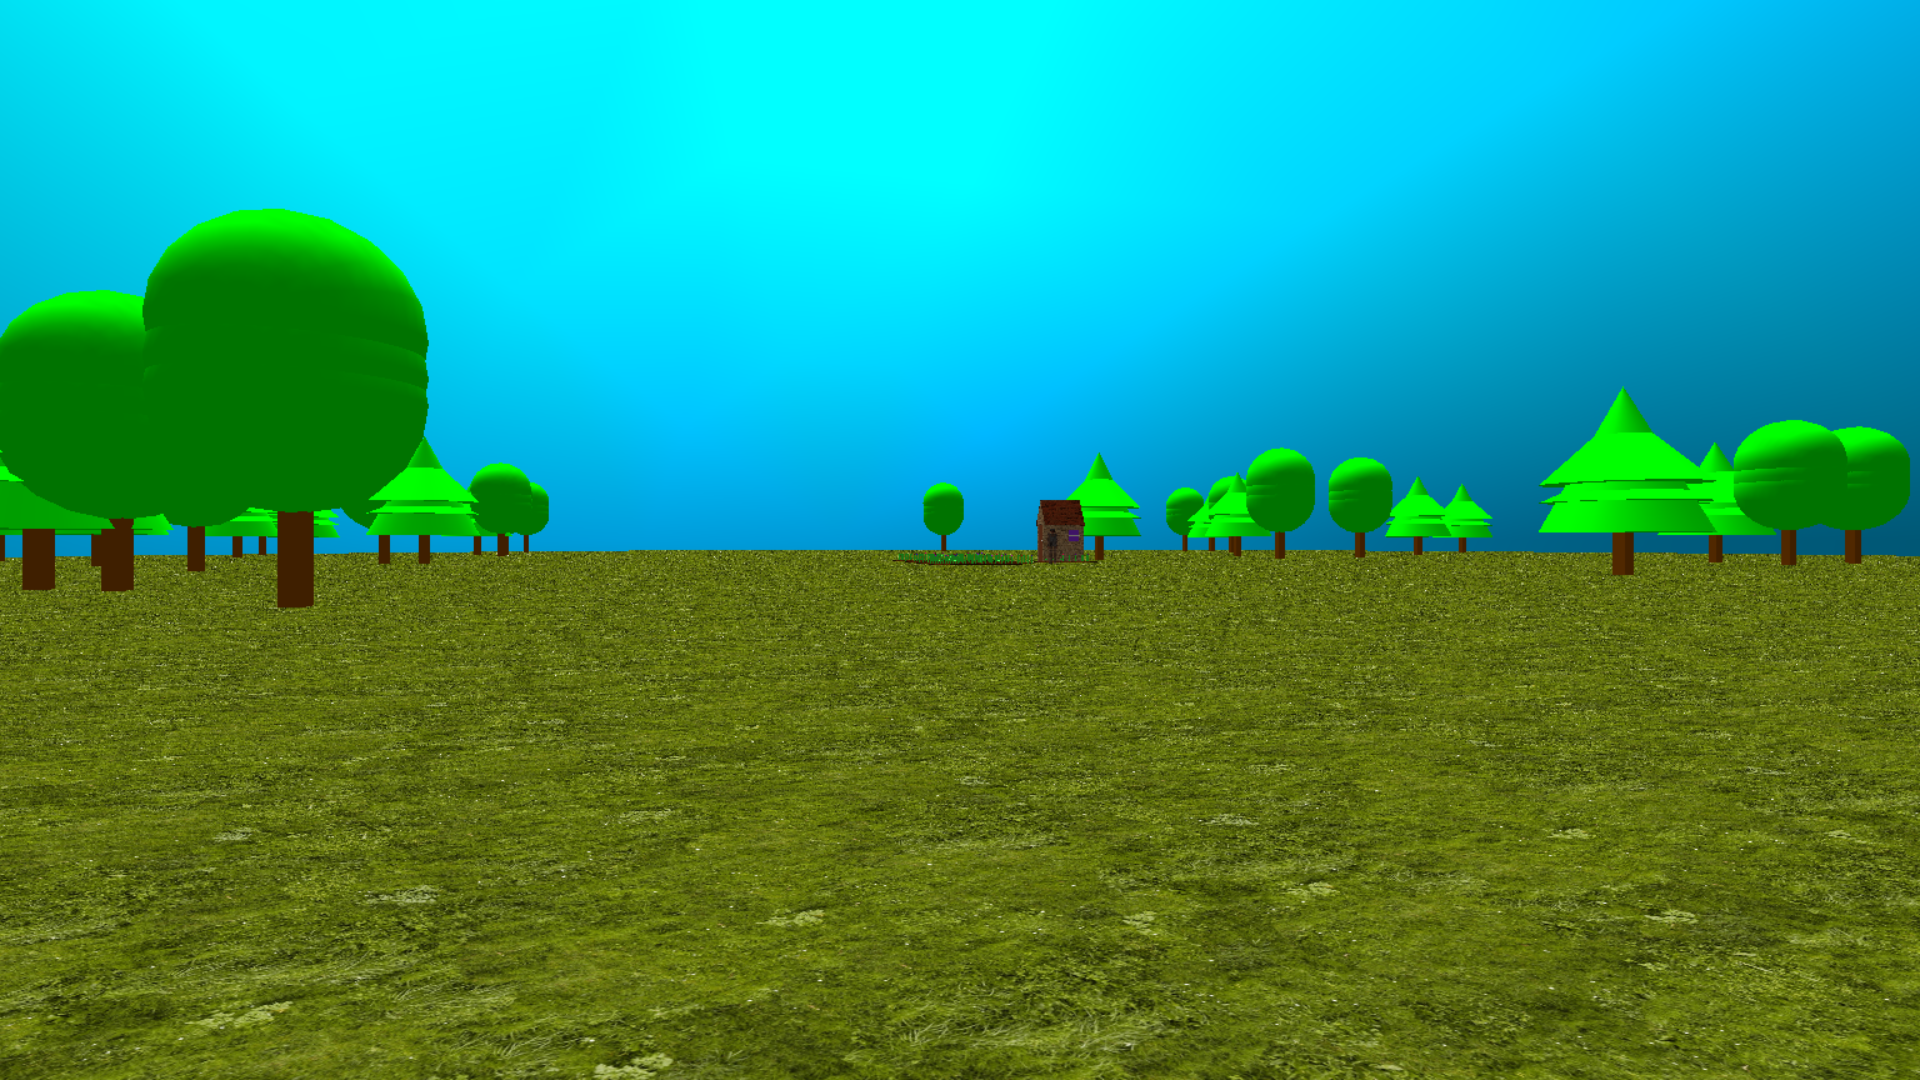
\includegraphics[scale=0.4]{imagens/cenario2.png}
\legend{Fonte: o autor}
\end{figure}


 Também foram implementadas as opções para se mover a câmera de acordo com algumas teclas, são elas 'a', 's', 'd', 'q', 'w' e 'e'. As teclas 'a' e 'd' fazem a câmera se mover para o lado esquerdo e direito respectivamente, as teclas 'w' e 's' fazem a câmera ir para frente e para trás respectivamente e as teclas 'q' e 'e' fazem a câmera girar no sentido anti-horário e horário respectivamente.




\chapter{Conclusão}

	Foi feito então um ambiente tridimensional baseado em um jogo de fazenda ao estilo minecraft, onde o personagem, no caso um fazendeiro, planta nos locais em que houveram \emph{clicks} do \emph{mause}. Para isso foi feita uma função que calcula o trajeto e os passos que o fazendeiro deverá executar. 

 Também foram feitos todos os objetos que constituem o cenário são eles as árvores, a casa, o solo e as plantas. Todos esses objetos foram criados apartir da combinação de figuras primitivas tais como cubos e esferas.  

Foi implementado também o menu que aparece quando há um \emph{click} do botão direito do mause, responsável por permitir ao usuário escolher se o personagem irá plantar, executar a animação automática ou qual parte do personagem mover. 

Foram feitas as animações do personagem plantando, dançando e andando. Essas animações foram armazenadas em filas que são percorridas afim de se executar a animação.

Também foram implementadas as opções de movimento da câmera ao se precionar determinadas teclas do teclado. E foram inseridas texturas  no personagem, no chão, no solo e na casa. Também foram definidas fontes de luz e suas especificações para iluminar os objetos.

Ao fim do desenvolvimento ficou mais claro como desenvolver uma aplicação gráfica e como funciona internamente um pacote gráfico como o opengl. Após algumas dificuldades para se fazer as animações  comprendeu-se melhor o processo de se animar objetos tridimensionais e a importância dos pequenos detalhes no resultado final das animações.
\nocite{NBR6028:2003}
  \nocite{vianna2001computaccao}
\nocite{pozzeropengl}
\nocite{woo1999opengl}
\nocite{wright2010opengl}
% ---
% Finaliza a parte no bookmark do PDF
% para que se inicie o bookmark na raiz
% e adiciona espaço de parte no Sumário
% ---
\phantompart


% ----------------------------------------------------------
% ELEMENTOS PÓS-TEXTUAIS
% ----------------------------------------------------------
\postextual

% ----------------------------------------------------------
% Referências bibliográficas
% ----------------------------------------------------------
\bibliography{referencias}


% ----------------------------------------------------------
% Apêndices
% ----------------------------------------------------------

% ---
% Inicia os apêndices
% ---


%---------------------------------------------------------------------
% INDICE REMISSIVO
%---------------------------------------------------------------------

\phantompart

\printindex


\end{document}
